\documentclass[tikz,border=2pt]{standalone}
\usepackage{amsmath}
\usetikzlibrary{arrows.meta}
\begin{document}
% Prisoner's Dilemma strategy sets S_1 = S_2 = {M, F}: the profile set S = S_1 x S_2 has 2*2 = 4
% cells. In the profile s = (F, M) we have s_1 = F, s_{-1} = M; the unilateral switch (s_1', s_{-1})
% to s_1' = M moves within the column s_{-1} = M, which stays fixed.
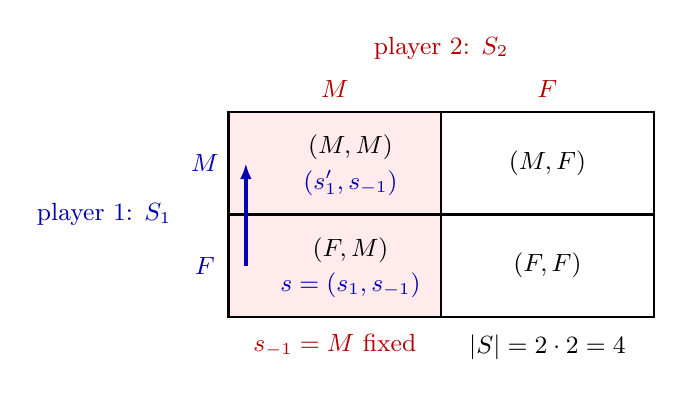
\begin{tikzpicture}[font=\small, >={Latex[length=2mm]}]
  \def\w{2.7} \def\h{1.3}
  % column s_{-1} = M held fixed
  \fill[red!8] (0,-\h) rectangle (\w,\h);
  \draw[thick] (0,-\h) rectangle (2*\w,\h);
  \draw[thick] (\w,-\h) -- (\w,\h);
  \draw[thick] (0,0) -- (2*\w,0);
  % strategy labels
  \node[red!70!black] at (0.5*\w,\h+0.3) {$M$};
  \node[red!70!black] at (1.5*\w,\h+0.3) {$F$};
  \node[blue!70!black] at (-0.3,0.5*\h) {$M$};
  \node[blue!70!black] at (-0.3,-0.5*\h) {$F$};
  \node[red!70!black, anchor=south] at (\w,\h+0.55) {player 2: $S_2$};
  \node[blue!70!black, anchor=east] at (-0.6,0) {player 1: $S_1$};
  % profiles
  \node at (0.5*\w+0.2,0.5*\h+0.2) {$(M,M)$};
  \node[blue!70!black] at (0.5*\w+0.2,0.5*\h-0.25) {$(s_1',s_{-1})$};
  \node at (1.5*\w,0.5*\h) {$(M,F)$};
  \node at (0.5*\w+0.2,-0.5*\h+0.2) {$(F,M)$};
  \node[blue!70!black] at (0.5*\w+0.2,-0.5*\h-0.25) {$s=(s_1,s_{-1})$};
  \node at (1.5*\w,-0.5*\h) {$(F,F)$};
  % unilateral switch of player 1
  \draw[->, very thick, blue!70!black] (0.22,-0.5*\h) -- (0.22,0.5*\h);
  % notes
  \node[red!70!black, anchor=north] at (0.5*\w,-\h-0.1) {$s_{-1}=M$ fixed};
  \node[anchor=north] at (1.5*\w,-\h-0.1) {$|S|=2\cdot2=4$};
\end{tikzpicture}
\end{document}
